\documentclass[12pt]{article}
\usepackage[utf8]{inputenc}
\usepackage{graphics}
\usepackage{graphicx}
\usepackage{float}
\usepackage{hyperref}
\usepackage{listings}
\lstset{
	basicstyle=\ttfamily,
	columns=fullflexible,
	frame=single,
	breaklines=true,
	postbreak=\mbox{\textcolor{red}{$\hookrightarrow$}\space},
}
\hypersetup{
	colorlinks=true,
	linkcolor=blue,
	filecolor=magenta,      
	urlcolor=cyan,
}

\title{OTAP opzetten}
\author{Thomas van Dongen, Koen Schilders}
\date{11 april 2018}

\begin{document}

% De titelpagina
\begin{titlepage}
\maketitle
\end{titlepage}

\section{Jenkins}
Om OTAP toe te voegen aan de ontwikkelstraat gaan we eerst een nieuw Jenkins project maken: het Production project. Dit project haalt de code van de git repository, en maakt een build zonder te testen.

\begin{figure}[H]
	\begin{center}
		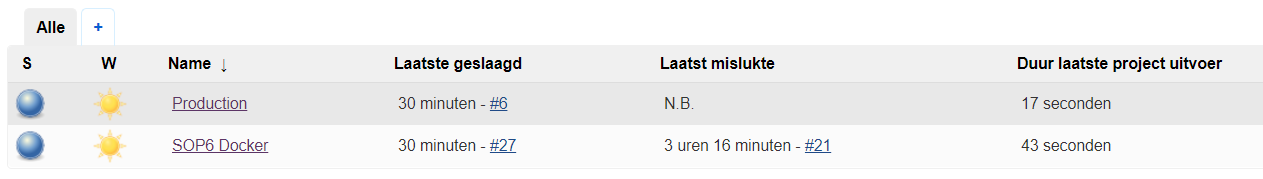
\includegraphics[width=0.75\textwidth]{images/jenkinsoverzicht.PNG}
		\caption{Beide projecten in Jenkins\label{fig:jenkinsoverzicht}}
	\end{center}
\end{figure}

In het SOP6 Docker project moet het Production project aangeroepen worden. Dit kan met de post-build action 'Bouw ander project'. Hier geven we aan dat we het Production project alleen willen starten als de build stabiel is.

\begin{figure}[H]
	\begin{center}
		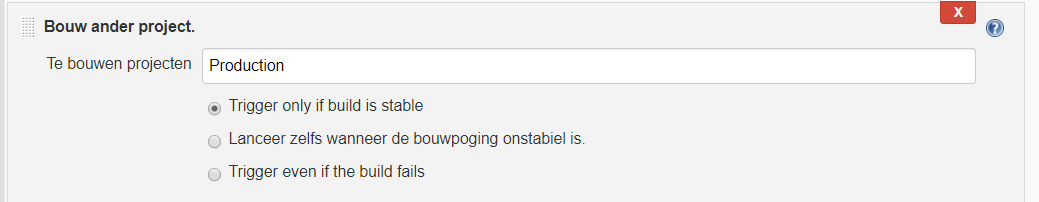
\includegraphics[width=0.75\textwidth]{images/post-build.PNG}
		\caption{Post-build action welke het Production-project aanroept\label{fig:post-build}}
	\end{center}
\end{figure}

De build wordt in een eigen folder op het host-systeem geplaatst. Na het builden zijn er twee plekken waar het project gebuild staat: de SOP6 Docker volume en de Production volume.

\section{Glassfish}
Nu we de productiebuild op het systeem hebben staan kunnen we een nieuwe Glassfish container aanmaken. Deze heeft andere poorten nodig, en het juiste volume moet gemapped worden. Dit wordt gedaan door het volgende commando:
\newline

\begin{lstlisting}[language=Bash]
docker run -i -t -p 4949:4848 -p 8182:8181 -v "/var/lib/docker/volumes/jenkins_home/_data/workspace/Production/target":/glassfish5/glassfish/domains/domain1/autodeploy oracle/glassfish:latest
\end{lstlisting}

Beide Glassfish containers kunnen naast elkaar draaien omdat ze op verschillende poorten zitten.

\begin{figure}[H]
	\begin{center}
		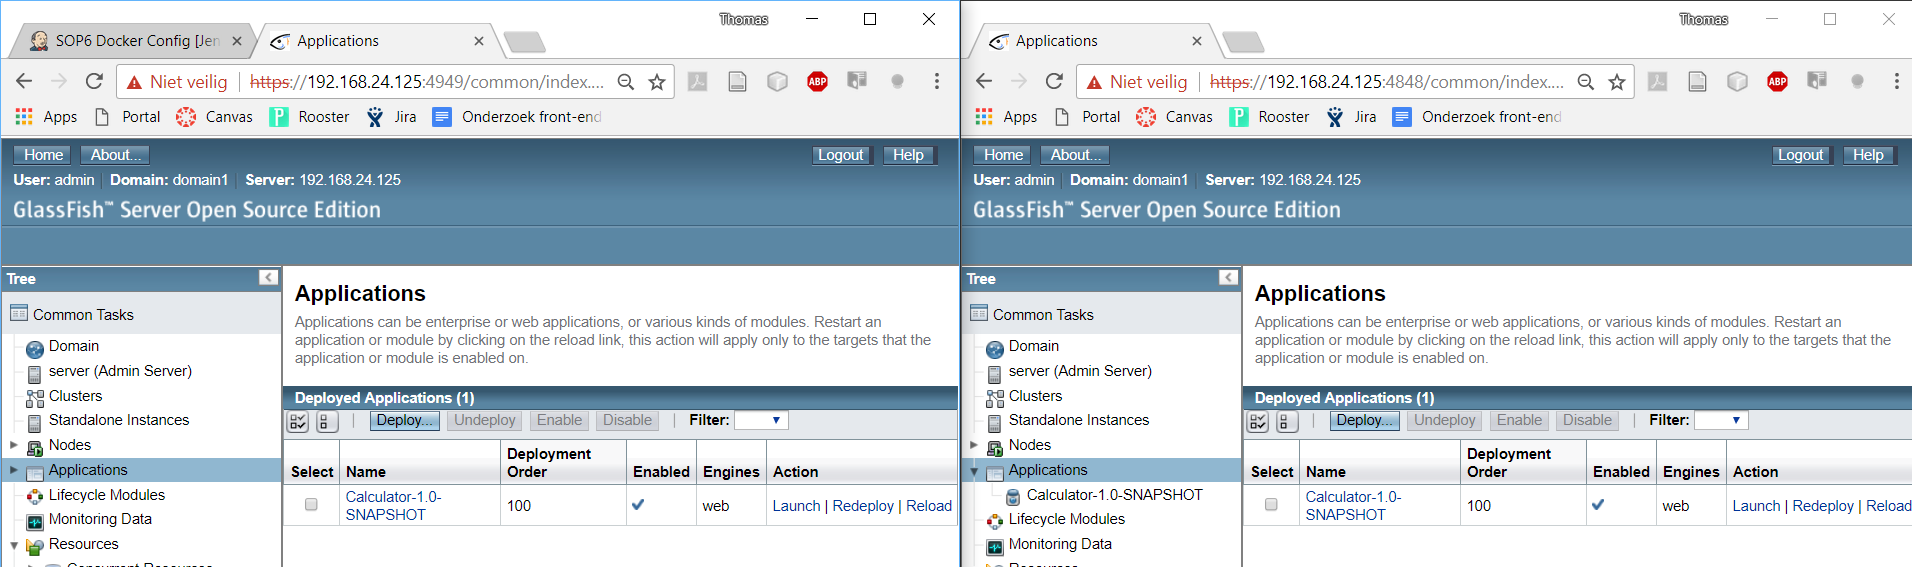
\includegraphics[width=0.75\textwidth]{images/glassfishomgevingen.PNG}
		\caption{Beide Glassfish omgevingen\label{fig:glassfishomgevingen}}
	\end{center}
\end{figure}

OTAP is nu succesvol opgezet. Zodra er een nieuwe build naar de master-branch van de git repository wordt gepushed, gaat Jenkins een nieuwe build maken. Deze build wordt uitvoerig getest, en wanneer deze succesvol is, wordt de build ook gestart voor production. Deze build wordt automatisch gehost, en is bereikbaar via de productie-url.

\end{document}